% Aberdeen style guide should be followed when using this
% layout. Their template powerpoint slide is used to extract the
% Aberdeen color and logo but is otherwise ignored (it has little or
% no formatting in it anyway).
%
% http://www.abdn.ac.uk/documents/style-guide.pdf

%%%%%%%%%%%%%%%%%%%% Document Class Settings %%%%%%%%%%%%%%%%%%%%%%%%%
% Pick if you want slides, or draft slides (no animations)
%%%%%%%%%%%%%%%%%%%%%%%%%%%%%%%%%%%%%%%%%%%%%%%%%%%%%%%%%%%%%%%%%%%%%%
%Normal document mode%
%\documentclass[10pt,compress]{beamer}
%Draft or handout mode
%\documentclass[10pt,compress,handout]{beamer}
\documentclass[10pt,compress,handout,ignorenonframetext]{beamer}

%%%%%%%%%%%%%%%%%%%% General Document settings %%%%%%%%%%%%%%%%%%%%%%%
% These settings must be set for each presentation
%%%%%%%%%%%%%%%%%%%%%%%%%%%%%%%%%%%%%%%%%%%%%%%%%%%%%%%%%%%%%%%%%%%%%%
\newcommand{\shortname}{jefferson.gomes@abdn.ac.uk}
\newcommand{\fullname}{Dr Jeff Gomes}
\institute{School of Engineering}
\newcommand{\emailaddress}{}%jefferson.gomes@abdn.ac.uk}
\newcommand{\logoimage}{../../FigBanner/UoAHorizBanner}
\title{Chemical Thermodynamics (EX3029)}
\subtitle{Module 3: Thermodynamic Properties of Pure Fluids}
\date[ ]{ }

%%%%%%%%%%%%%%%%%%%% Template settings %%%%%%%%%%%%%%%%%%%%%%%%%%%%%%%
% You shouldn't have to change below this line, unless you want to.
%%%%%%%%%%%%%%%%%%%%%%%%%%%%%%%%%%%%%%%%%%%%%%%%%%%%%%%%%%%%%%%%%%%%%%
\usecolortheme{whale}
\useoutertheme{infolines}

% Use the fading effect for items that are covered on the current
% slide.
\beamertemplatetransparentcovered

% We abuse the author command to place all of the slide information on
% the title page.
\author[\shortname]{%
  \fullname\\\ttfamily{\emailaddress}
}


%At the start of every section, put a slide indicating the contents of the current section.
\AtBeginSection[] {
  \begin{frame}
    \frametitle{Section Outline}
    \tableofcontents[currentsection]
  \end{frame}
}

% Allow the inclusion of movies into the Presentation! At present,
% only the Okular program is capable of playing the movies *IN* the
% presentation.
\usepackage{multimedia}
\usepackage{animate}

%% Handsout -- comment out the lines below to create handstout with 4 slides in a page with space for comments
\usepackage{handoutWithNotes}

\mode<handout>
{
\usepackage{pgf,pgfpages}

\pgfpagesdeclarelayout{2 on 1 boxed with notes}
{
\edef\pgfpageoptionheight{\the\paperheight} 
\edef\pgfpageoptionwidth{\the\paperwidth}
\edef\pgfpageoptionborder{0pt}
}
{
\setkeys{pgfpagesuselayoutoption}{landscape}
\pgfpagesphysicalpageoptions
    {%
        logical pages=4,%
        physical height=\pgfpageoptionheight,%
        physical width=\pgfpageoptionwidth,%
        last logical shipout=2%
    } 
\pgfpageslogicalpageoptions{1}
    {%
    border code=\pgfsetlinewidth{1pt}\pgfstroke,%
    scale=1,
    center=\pgfpoint{.25\pgfphysicalwidth}{.75\pgfphysicalheight}%
    }%
\pgfpageslogicalpageoptions{2}
    {%
    border code=\pgfsetlinewidth{1pt}\pgfstroke,%
    scale=1,
    center=\pgfpoint{.25\pgfphysicalwidth}{.25\pgfphysicalheight}%
    }%
\pgfpageslogicalpageoptions{3}
    {%
    border shrink=\pgfpageoptionborder,%
    resized width=.7\pgfphysicalwidth,%
    resized height=.5\pgfphysicalheight,%
    center=\pgfpoint{.75\pgfphysicalwidth}{.29\pgfphysicalheight},%
    copy from=3
    }%
\pgfpageslogicalpageoptions{4}
    {%
    border shrink=\pgfpageoptionborder,%
    resized width=.7\pgfphysicalwidth,%
    resized height=.5\pgfphysicalheight,%
    center=\pgfpoint{.75\pgfphysicalwidth}{.79\pgfphysicalheight},%
    copy from=4
    }%

\AtBeginDocument
    {
    \newbox\notesbox
    \setbox\notesbox=\vbox
        {
            \hsize=\paperwidth
            \vskip-1in\hskip-1in\vbox
            {
                \vskip1cm
                Notes\vskip1cm
                        \hrule width\paperwidth\vskip1cm
                    \hrule width\paperwidth\vskip1cm
                        \hrule width\paperwidth\vskip1cm
                    \hrule width\paperwidth\vskip1cm
                        \hrule width\paperwidth\vskip1cm
                    \hrule width\paperwidth\vskip1cm
                    \hrule width\paperwidth\vskip1cm
                    \hrule width\paperwidth\vskip1cm
                        \hrule width\paperwidth
            }
        }
        \pgfpagesshipoutlogicalpage{3}\copy\notesbox
        \pgfpagesshipoutlogicalpage{4}\copy\notesbox
    }
}
}

\pgfpagesuselayout{2 on 1 boxed with notes}[letterpaper,border shrink=5mm]

%%%%% Color settings
\usepackage{color}
%% The background color for code listings (i.e. example programs)
\definecolor{lbcolor}{rgb}{0.9,0.9,0.9}%
\definecolor{UoARed}{rgb}{0.64706, 0.0, 0.12941}
\definecolor{UoALight}{rgb}{0.85, 0.85, 0.85}
\definecolor{UoALighter}{rgb}{0.92, 0.92, 0.92}
\setbeamercolor{structure}{fg=UoARed} % General background and higlight color
\setbeamercolor{frametitle}{bg=black} % General color
\setbeamercolor{frametitle right}{bg=black} % General color
\setbeamercolor{block body}{bg=UoALighter} % For blocks
\setbeamercolor{structure}{bg=UoALight} % For blocks
% Rounded boxes for blocks
\setbeamertemplate{blocks}[rounded]

%%%%% Font settings
% Aberdeen requires the use of Arial in slides. We can use the
% Helvetica font as its widely available like so
% \usepackage{helvet}
% \renewcommand{\familydefault}{\sfdefault}
% But beamer already uses a sans font, so we will stick with that.

% The size of the font used for the code listings.
\newcommand{\goodsize}{\fontsize{6}{7}\selectfont}

% Extra math packages, symbols and colors. If you're using Latex you
% must be using it for formatting the math!
\usepackage{amscd,amssymb} \usepackage{amsfonts}
\usepackage[mathscr]{eucal} \usepackage{mathrsfs}
\usepackage{latexsym} \usepackage{amsmath} \usepackage{bm}
\usepackage{amsthm} \usepackage{textcomp} \usepackage{eurosym}
% This package provides \cancel{a} and \cancelto{a}{b} to "cancel"
% expressions in math.
\usepackage{cancel}

\usepackage{comment} 

% Get rid of font warnings as modern LaTaX installations have scalable
% fonts
\usepackage{type1cm} 

%\usepackage{enumitem} % continuous numbering throughout enumerate commands

% For exact placement of images/text on the cover page
\usepackage[absolute]{textpos}
\setlength{\TPHorizModule}{1mm}%sets the textpos unit
\setlength{\TPVertModule}{\TPHorizModule} 

% Source code formatting package
\usepackage{listings}%
\lstset{ backgroundcolor=\color{lbcolor}, tabsize=4,
  numberstyle=\tiny, rulecolor=, language=C++, basicstyle=\goodsize,
  upquote=true, aboveskip={1.5\baselineskip}, columns=fixed,
  showstringspaces=false, extendedchars=true, breaklines=false,
  prebreak = \raisebox{0ex}[0ex][0ex]{\ensuremath{\hookleftarrow}},
  frame=single, showtabs=false, showspaces=false,
  showstringspaces=false, identifierstyle=\ttfamily,
  keywordstyle=\color[rgb]{0,0,1},
  commentstyle=\color[rgb]{0.133,0.545,0.133},
  stringstyle=\color[rgb]{0.627,0.126,0.941}}

% Allows the inclusion of other PDF's into the final PDF. Great for
% attaching tutorial sheets etc.
\usepackage{pdfpages}
\setbeamercolor{background canvas}{bg=}  

% Remove foot note horizontal rules, they occupy too much space on the slide
\renewcommand{\footnoterule}{}

% Force the driver to fix the colors on PDF's which include mixed
% colorspaces and transparency.
\pdfpageattr {/Group << /S /Transparency /I true /CS /DeviceRGB>>}

% Include a graphics, reserve space for it but
% show it on the next frame.
% Parameters:
% #1 Which slide you want it on
% #2 Previous slides
% #3 Options to \includegraphics (optional)
% #4 Name of graphic
\newcommand{\reserveandshow}[4]{%
\phantom{\includegraphics<#2|handout:0>[#3]{#4}}%
\includegraphics<#1>[#3]{#4}%
}

\newcommand{\frc}{\displaystyle\frac}
\newcommand{\red}{\textcolor{red}}
\newcommand{\blue}{\textcolor{blue}}
\newcommand{\green}{\textcolor{green}}
\newcommand{\purple}{\textcolor{purple}}
 
\begin{document}

% Title page layout
\begin{frame}
  \titlepage
  \vfill%
  \begin{center}
    \includegraphics[clip,width=0.8\textwidth]{\logoimage}
  \end{center}
\end{frame}

% Table of contents
\frame{ \frametitle{Slides Outline}
  \tableofcontents
}


%%%%%%%%%%%%%%%%%%%% The Presentation Proper %%%%%%%%%%%%%%%%%%%%%%%%%
% Fill below this line with \begin{frame} commands! It's best to
% always add the fragile option incase you're going to use the
% verbatim environment.
%%%%%%%%%%%%%%%%%%%%%%%%%%%%%%%%%%%%%%%%%%%%%%%%%%%%%%%%%%%%%%%%%%%%%%


%%%
%%% SECTION
%%%
%\section{General Remarks}

%%%
%%% Slides
%%%
\begin{frame}
 \frametitle{Aims and Objectives}
   \begin{enumerate}
     \item<1-> In Modules 1-3, we learnt:
       \begin{enumerate}
         \item<1-> the laws of Thermodynamics and how they describe thermal equilibrium of species in closed and opened systems;
         \item<1-> how to calculate thermodynamics properties -- internal energy, enthalpy and entropy for pure chemicallspecies;
         \item<1-> PVT behaviour of pure species in equilibrium and;
         \item<1-> Equations of state.
       \end{enumerate} 
     \item<2-> This Module focuses on 
         \begin{enumerate}
           \item<2-> Thermodynamic properties of pure fluids;
           \item<2-> Introduce two remaining thermodynamic properties: Gibbs and Helmholtz free energies;
           \item<2-> Maxwell relations.
         \end{enumerate}
   \end{enumerate}

\end{frame}


%%%
%%% SECTION
%%%
%\section{Bibliography}
\begin{frame}
 \frametitle{Suggested References}
  Literature relevant for this module:
  \begin{enumerate}[(a)]
   \item\label{SVN_Book} J.M. Smith, H.C. Van Ness, M.M. Abbott, $\lq$Introduction to Chemical Engineering Thermodynamics', 6$^{th}$ Edition: Chapter 6;
   \item Y.A. Cengel, M.A. Boles, $\lq$Thermodynamics -- An Engineering Approach', 5$^{th}$ Edition: Chapter 12.1-4; 
   %\item M.J. Moran, H.N. Saphiro, D.D. Boettner, M.B. Bailey, $\lq$Principles of Engineering Thermodynamics', 7$^{th}$ Edition: Chapters 3;
   %\item C. Borgnakke, R.E. Sonntag,$\lq$Fundamentals of Thermodynamics',8$^{th}$ Edition: Chapter 2.
   \item S.I. Sandler, $\lq$Chemical, Biochemical and Engineering Thermodynamics', 4$^{th}$ Edition: Chapter 6.
  \end{enumerate}
\end{frame}


%%%
%%% SECTION
%%%
\section{Property Relations for Homogeneous Phases}

%%%
%%% SUBSECTION
%%%
\subsection{Thermodynamic Potentials} 


%%%
%%% Slide
%%%
%\scriptsize
\begin{frame}
  \frametitle{New State Functions}
   \visible<1->{\begin{block}{Enthalpy}
      \begin{displaymath}
         H = U + P V
      \end{displaymath}
   \end{block}
   }
   \visible<2->{\begin{block}{Gibbs Free Energy}
      \begin{displaymath}
         G = H - T S
      \end{displaymath}
   \end{block}
   }
   \visible<3->{\begin{block}{Helmholtz Free Energy}
      \begin{displaymath}
         A = U - T S
      \end{displaymath}
   \end{block}
   }

\end{frame}
\normalsize

%%%
%%% SUBSECTION
%%%
\subsection{Maxwell's Relations}
%%%
%%% Slide
%%%
%\scriptsize
\begin{frame}
  \frametitle{Maxwell's Relations}
   \visible<1->{\begin{block}{For 1 mol of homogeneous fluid at $T=$ constant}
      \begin{center}
        \begin{tabular}{l c  l}
           $sU = T dS - PdV$  &  \hspace{1cm} & $dH = TdS + VdP$ \\
           $dA = -PdV - SdT$  &  \hspace{1cm} & $dG = VdP - SdT$ 
        \end{tabular}
      \end{center}
   \end{block}
   }
   \visible<2->{\begin{block}{Maxwell's Equations}
      \begin{center}
        \begin{tabular}{l c  l}
           $\left(\frc{\partial T}{\partial V}\right)_{S} = -\left(\frc{\partial P}{\partial S}\right)_{v}$  &  \hspace{1cm} & $\left(\frc{\partial T}{\partial P}\right)_{S} =  \left(\frc{\partial V}{\partial S}\right)_{P}$  \\
           $\left(\frc{\partial P}{\partial T}\right)_{V} =  \left(\frc{\partial S}{\partial V}\right)_{T}$  &  \hspace{1cm} & $\left(\frc{\partial V}{\partial T}\right)_{S} = -\left(\frc{\partial S}{\partial P}\right)_{T}$ 
        \end{tabular}
      \end{center}
   \end{block}
   }

\end{frame}
\normalsize


%%%
%%% SUBSECTION
%%%
\subsection{Thermodynamic Potentials: Dependence on $T$ and $P$}

%%%
%%% Slide
%%%
%\scriptsize
\begin{frame}
  \frametitle{Internal Energy, Enthalpy and Entropy}
   \visible<1->{\begin{block}{$H$ and $S$ as functions of $T$ and $P$}
      \begin{center}
        \begin{tabular}{l c  l}
           $dH = C_{p}dT + \left[ V - T\left(\frc{\partial V}{\partial T}\right)_{P}\right]dP$ &  \hspace{1cm} & $dS=C_{p}\frc{dT}{T} - \left(\frc{\partial V}{\partial T}\right)_{P}dP$
        \end{tabular}
      \end{center}
   \end{block}
   }
   \visible<2->{\begin{block}{Ideal Gas}
      \begin{center}
        \begin{tabular}{l c  l}
           $dH = C_{p}dT$  &  \hspace{1cm} & $dS=C_{p}\frc{dT}{T} - R\frc{dP}{P}$  
        \end{tabular}
      \end{center}
   \end{block}
   }
   \visible<3->{\begin{block}{Liquid}
      \begin{center}
        \begin{tabular}{l c  l}
           $dH = C_{p}dT + \left(1-\beta\right)VdP$  &  \hspace{1cm} & $dS = C_{p}\frc{dT}{T} - \beta V{dP}$  
        \end{tabular}
      \end{center}
   \end{block}
   }
   \visible<4->{\begin{block}{$U$ and $S$ as functions of $T$ and $V$}
      \begin{center}
        \begin{tabular}{l c  l}
           $dU = C_{v}dT + \left[T\left(\frc{\partial P}{\partial T}\right)_{V} - P\right]dV$  &  \hspace{1cm} & $dS = C_{v}\frc{dT}{T} - \left(\frc{\partial P}{\partial T}\right)_{V}dV$  
        \end{tabular}
      \end{center}
   \end{block}
   }

\end{frame}
\normalsize


%%%
%%% Slide
%%%
%\scriptsize
\begin{frame}
  \frametitle{Gibbs Free Energy as Differential Operator}
     \begin{enumerate}[(a)]
        \item<1-> Gibbs Energy as generating function:
              \begin{displaymath}
                 \visible<1->{dG = VdP - SdT} \visible<2->{\Longrightarrow d\left(\frc{G}{RT}\right) = \frc{1}{RT}dG - \frc{G}{RT^{2}}dT} \nonumber 
              \end{displaymath}

        \item<3-> After substitution $\&$ algebraic reduction:
              \begin{displaymath}
                  \visible<3->{\frc{V}{RT} = \left\{ \frc{\partial\left(\frc{G}{RT}\right)}{\partial P}\right\}_{T} \hspace{1cm}\text{and}\hspace{1cm} \frc{H}{RT} = -T\left\{ \frc{\partial\left(\frc{G}{RT}\right)}{\partial T}\right\}_{P}}
              \end{displaymath}

        \item<4-> \textcolor{blue}{The Gibbs free energy when expressed as $G\left(T,P\right)$ operates as a generating function for other thermodynamic properties, and implicitly represents complete property information.}
     \end{enumerate}

\end{frame}
\normalsize

%%%
%%% SECTION
%%%
\section{Residual Properties}

\subsection{General Approach}
%%%
%%% Slide
%%%
%\scriptsize
\begin{frame}
  \frametitle{Residual Properties: General Approach}
     \begin{enumerate}[(a)]
        \item<1-> \textcolor{blue}{Residual Gibbs energy} is defined as:
              \visible<1->{\begin{displaymath}
                 \textcolor{red}{G^{R} = G - G^{ig}}
              \end{displaymath}}
            where \textcolor{blue}{$G$} is the actual Gibbs energy and \textcolor{blue}{$G^{id}$} is the correspondent thermodynamic function for ideal gas at same $T$ and $P$;
        \item<2-> This leads to,
              \visible<2->{\begin{displaymath}
                 d\left(\frc{G^{R}}{RT}\right) =\frc{V^{R}}{RT}dP - \frc{H^{R}}{RT^{2}}dT
              \end{displaymath}}
             
              \visible<3->{with,\begin{displaymath}
                 \frc{V^{R}}{RT} = \left\{ \frc{\partial\left(\frc{G^{R}}{RT}\right)}{\partial P}\right\}_{T} \hspace{0.5cm}\text{ and }\hspace{0.5cm} \frc{H^{R}}{RT} = -T\left\{ \frc{\partial\left(\frc{G^{R}}{RT}\right)}{\partial T}\right\}_{P}
              \end{displaymath}}
     \end{enumerate}

\end{frame}
\normalsize


%%%
%%% SUBSECTION
%%%
\subsection{Equations of State}
%%%
%%% Slide
%%%
%\scriptsize
\begin{frame}
  \frametitle{Residual Properties by EOS}
       Alternative approach to numerical integration: analytical solution by EOS:
            \begin{enumerate}[(a)]
                \item<1-> Virial EOS: \textcolor{blue}{$Z = 1 + \frc{BP}{RT}$}, 
                   \visible<2->{leading to \begin{displaymath}
                      \frc{G^{R}}{RT} = \displaystyle\int\limits_{0}^{\rho}\left(Z - 1\right)\frc{d\rho}{\rho} + Z - 1 - \ln Z \hspace{1cm} \frc{H^{R}}{RT} = -T \displaystyle\int\limits_{0}^{\rho}\left(\frc{\partial Z}{\partial T}\right)_{\rho}\frc{d\rho}{\rho} + Z - 1
                   \end{displaymath}
                   \begin{displaymath}
                      \frc{S^{R}}{RT} = \ln Z - T \displaystyle\int\limits_{0}^{\rho} \left(\frc{\partial Z}{\partial T}\right)_{\rho} \frc{d\rho}{\rho} - \displaystyle\int\limits_{0}^{\rho}\left(Z - 1\right)\frc{d\rho}{\rho} 
                   \end{displaymath}
}
             \end{enumerate}
\end{frame}
\normalsize



%%%
%%% Slide
%%%
%\scriptsize
\begin{frame}
  \frametitle{Residual Properties by EOS}
            \begin{enumerate}[(a)]\setcounter{enumi}{1}
               \item<1-> Cubic EOS: \textcolor{blue}{$P = \frc{RT}{V - b} - \frc{a\left(T\right)}{\left(V + \epsilon b\right)\left(V + \sigma b\right)}$}
                   \visible<2->{leading to\begin{displaymath}
                      \frc{G^{R}}{RT} = Z - 1 - \ln\left(Z - \beta\right) - q\mathcal{I} \hspace{1cm} \frc{H^{R}}{RT} = Z - 1 + \left[\frc{d\ln\alpha\left(T_{r}\right)}{d\ln T_{r}} - 1\right]q\mathcal{I}
                   \end{displaymath}
                   \begin{displaymath}
                       \frc{S^{R}}{R} = \ln\left(Z - \beta \right) + \frc{d\ln\alpha\left(T_{r}\right)}{d\ln T_{r}}q\mathcal{I} 
                   \end{displaymath}
                   with
                   \begin{displaymath}
                      \mathcal{I} \equiv \displaystyle\int\limits_{0}^{P} \frc{d\left(\rho b\right)}{\left(1 + \epsilon\rho b\right)\left(1 + \sigma\rho b\right)}\;\;\;\;\left(T\text{ const.}\right)
                   \end{displaymath}
                   See Section 6.3 of Smith, Van Ness $\&$ Abbott -- \textcolor{blue}{Reference (\ref{SVN_Book})}.
}
             \end{enumerate}

\end{frame}
\normalsize





%%%
%%% SECTION
%%%
\section{Two-Phase Systems}

\subsection{General Remarks}
%%%
%%% Slide
%%%
%\scriptsize
\begin{frame}
  \frametitle{General Remarks}
     \begin{enumerate}[(a)]
         \item<1-> \textcolor{blue}{Phase transition}: many extensive properties change abruptly during phase transition at given $P$ and $T$: specific volume, internal energy, enthalpy and entropy;
         \item<2-> \textcolor{blue}{Exception:} \textcolor{red}{molar Gibbs energy};
         \item<3-> For 2 phases \textcolor{blue}{$\alpha$} and \textcolor{blue}{$\beta$} of pure species at equilibrium,
            \visible<3->{\begin{block}{\textcolor{blue}{Equilibrium $\Rightarrow$ Equality of Gibbs energy}}
                     \begin{displaymath}
                        \textcolor{red}{G^{\alpha} = G^{\beta}} 
                     \end{displaymath}
            \end{block}}
         \item<4-> Clapeyron equation:
            \visible<4->{\begin{displaymath}
              \frc{d P^{sat}}{d T} = \frc{\Delta H^{lv}}{T \Delta V^{lv}}
            \end{displaymath}}
     \end{enumerate}

\end{frame}
\normalsize


%%%
%%% Slide
%%%
%\scriptsize
\begin{frame}
  \frametitle{General Remarks}
     \begin{enumerate}[(a)]\setcounter{enumi}{4}
         \item<1-> Temperature dependence of vapour pressure \blue{$\Rightarrow$} Empirical approaches for practical applications:
         \begin{enumerate}[(i)]
            \item<2-> Simplest case:
                \visible<2->{\begin{displaymath}
                   \ln P^{sat} = A - \frc{B}{T}
                \end{displaymath}}
            \item<3-> Antoine Equation:
                \visible<3->{\begin{displaymath}
                   \ln P^{sat} = A - \frc{B}{T+C}
                \end{displaymath}}
            \item<4-> Wagner Equation \blue{(more accurate)}:
                \visible<4->{\begin{displaymath}
                   \ln P_{r}^{sat} = \frc{A\tau + B\tau^{1.5} + C\tau^{3} + D\tau^{6}}{1-\tau}\;\;\;\text{ with }\;\;\; \tau = 1 - T_{r}
                \end{displaymath}}
         \end{enumerate}
     \end{enumerate}

\end{frame}
\normalsize


%%%
%%% SUBSECTION 
%%%
\subsection{Liquid/Vapour Systems}
%%%
%%% Slide
%%%
%\scriptsize
\begin{frame}
  \frametitle{Liquid/Vapour Systems}
     \begin{enumerate}[(a)]
         \item<1-> Systems with \blue{saturated vapour} and \blue{saturated liquid} in \red{equilibrium};
         \item<2-> \blue{Mass/Energy Balance} for any extensive property:
            \visible<3->{\begin{displaymath} 
                nV = n^{(l)}V^{(l)} + n^{(v)}V^{(v)} \;\;\; \Leftrightarrow \;\;\; V = x^{(l)}V^{(l)} + x^{(v)}V^{(v)}
             \end{displaymath}
             where $x^{(j)}$ is the \blue{molar/mass fraction} of phase \blue{j = l, v} $\rightarrow$  $x^{(l)} + x^{(v)} = 1$. 
            }
         \item<4-> The mass/molar volume fraction of vapour, \blue{$x^{(v)}$}, is also called \blue{vapour quality}. 
     \end{enumerate}

\end{frame}
\normalsize


%%%
%%%
%%% SUBSECTION 
%%%
\subsection{Thermodynamic Diagrams}

%%%
%%% Slide
%%%
%\scriptsize
\begin{frame}
  \frametitle{Pressure $\times$ Enthalpy ({\it PH}) Diagram}
      \begin{figure}%
        \begin{center}
          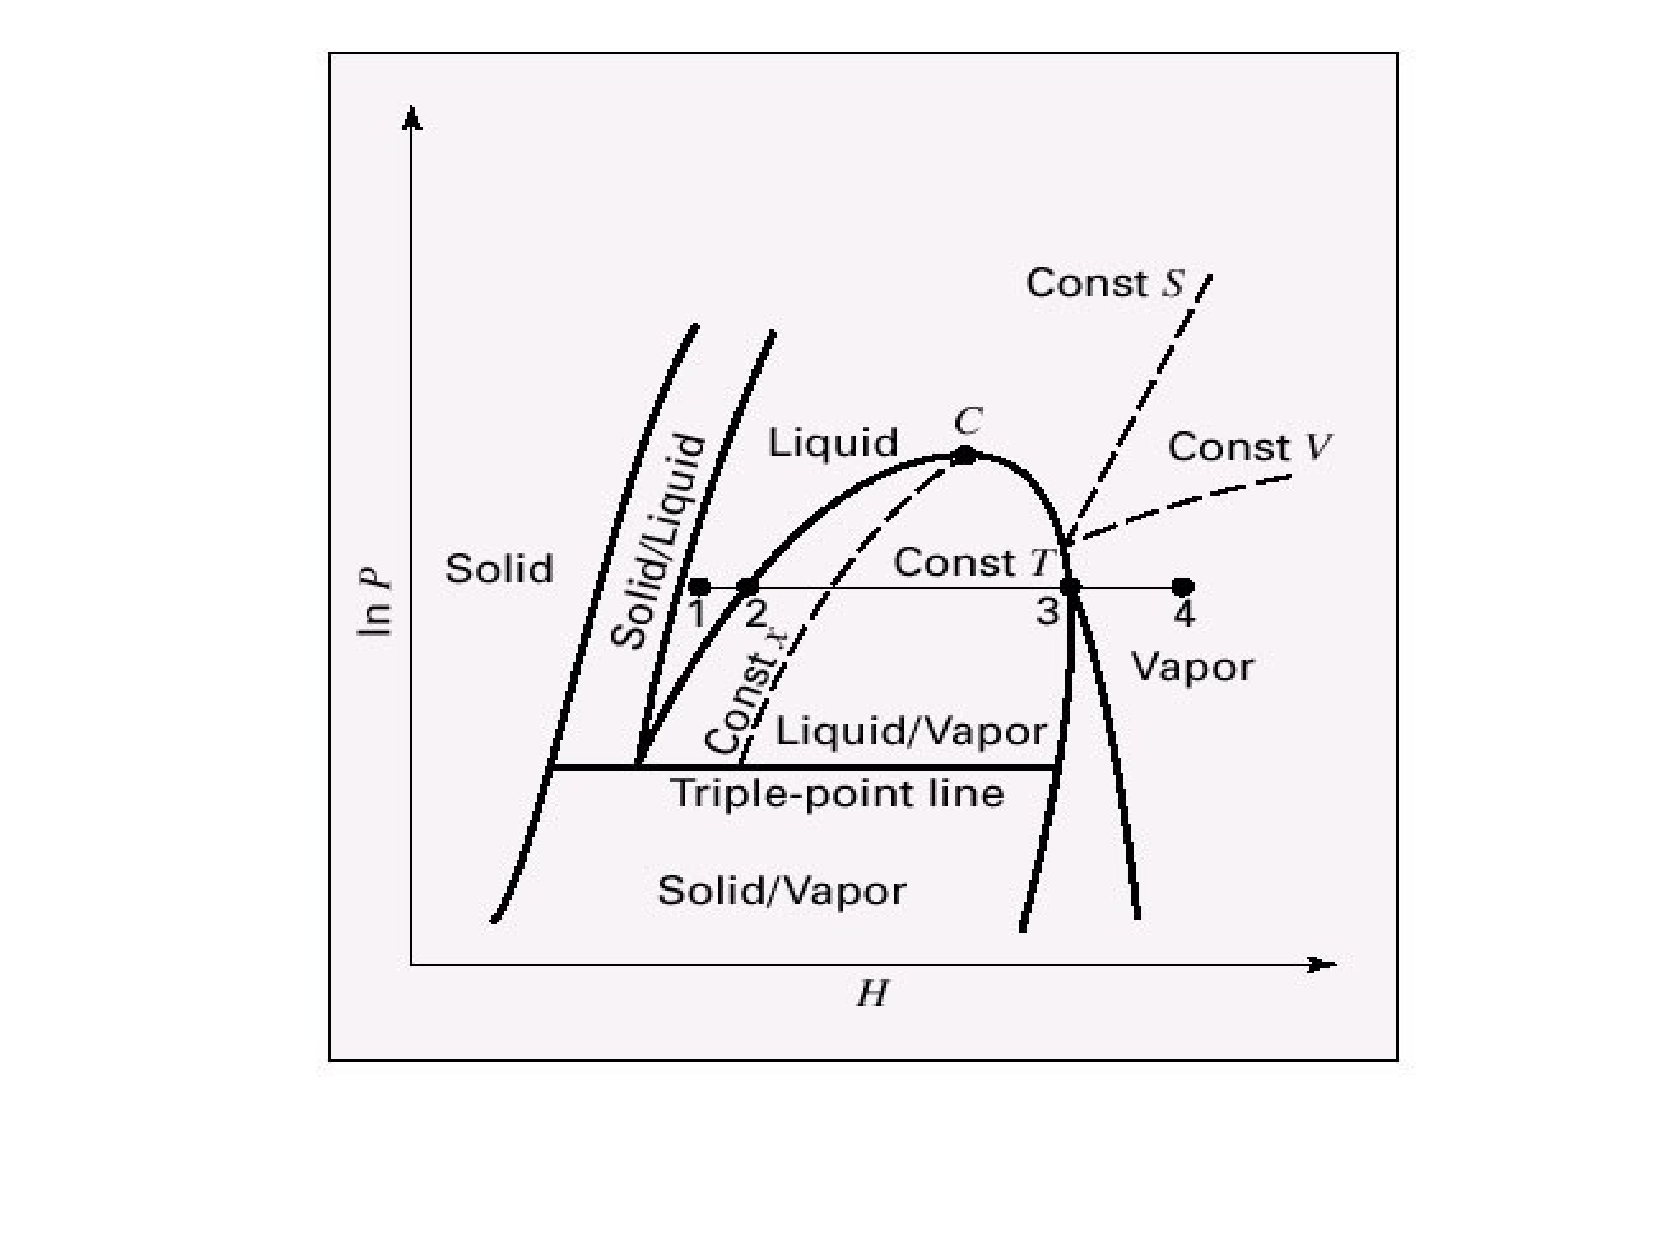
\includegraphics[width=1\columnwidth,clip]{./Pics/LnP_H_Diagram}
        \end{center}
      \end{figure}
\end{frame}
\normalsize


%%%
%%% Slide
%%%
%\scriptsize
\begin{frame}
  \frametitle{Temperature $\times$ Entropy ({\it TS}) Diagram}
      \begin{figure}%
        \begin{center}
          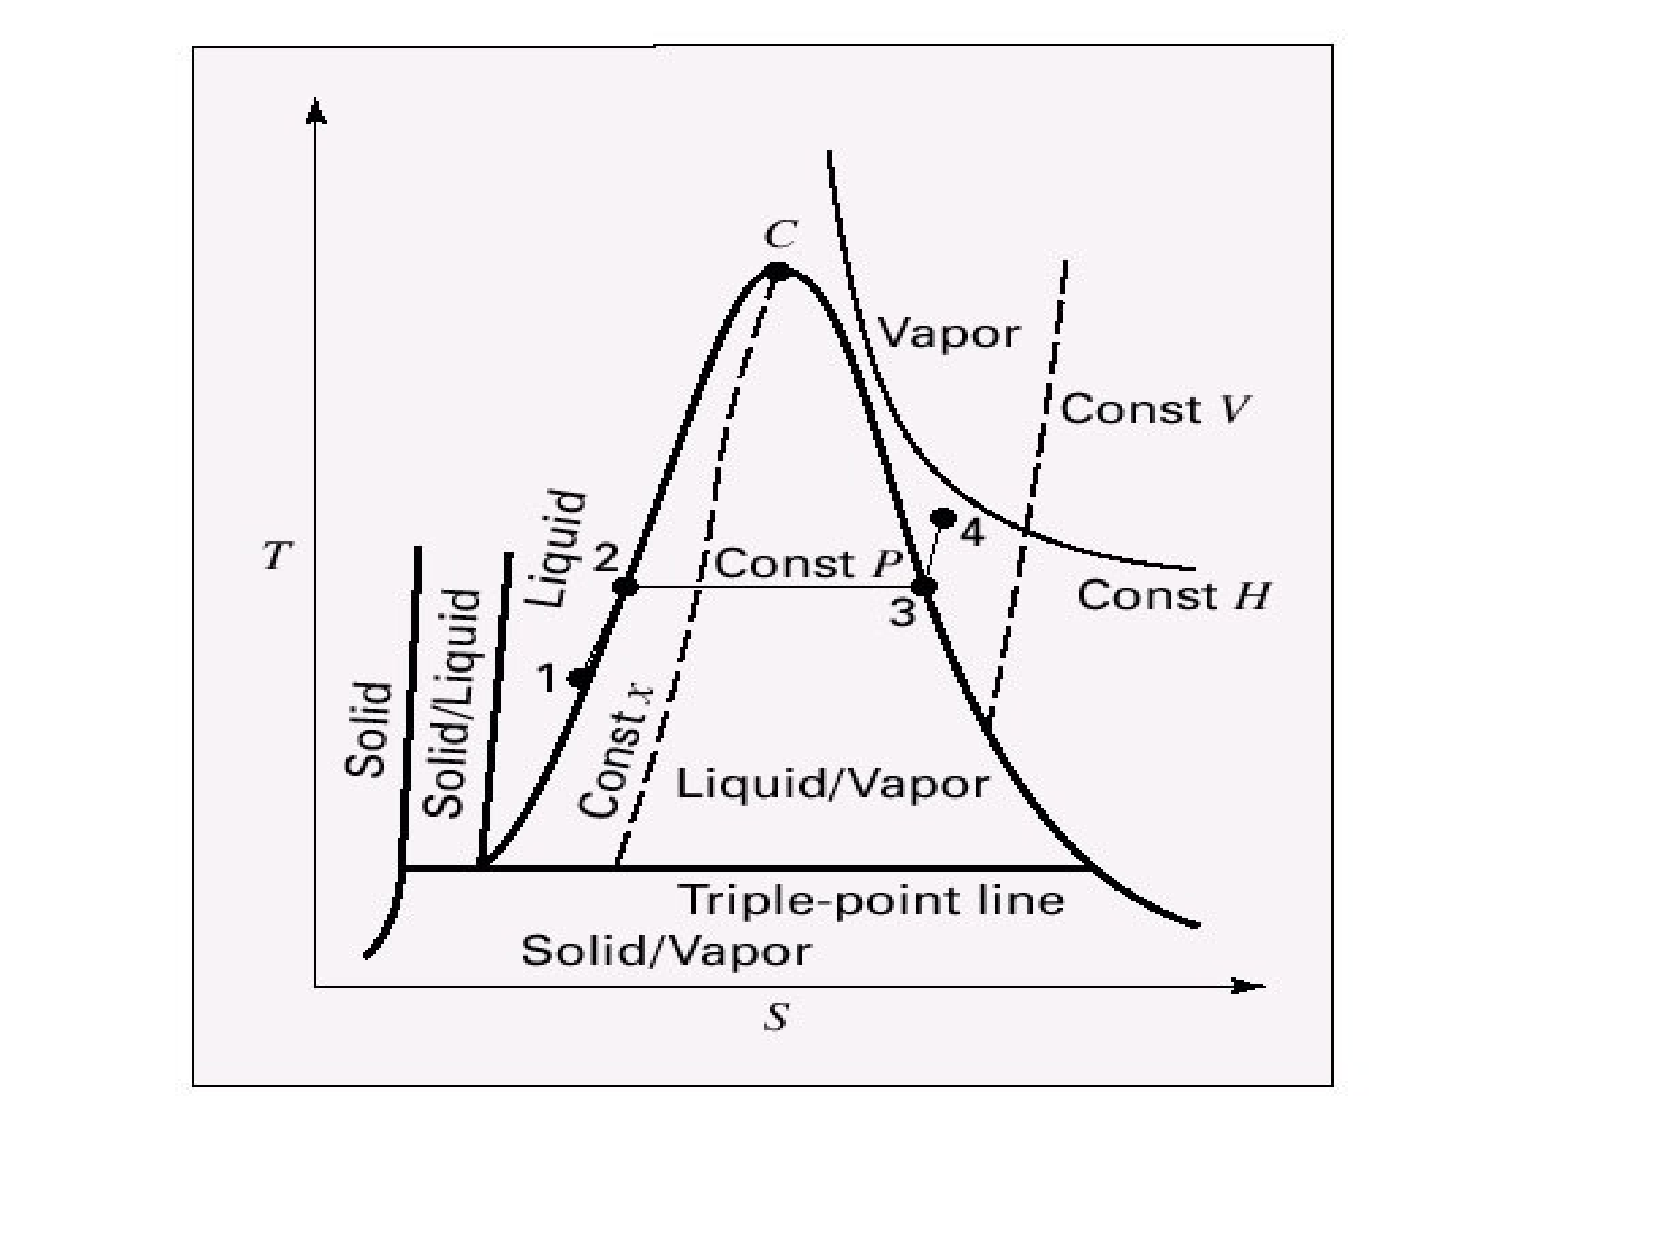
\includegraphics[width=1\columnwidth,clip]{./Pics/T_S_Diagram}
        \end{center}
      \end{figure}
\end{frame}
\normalsize

%%%
%%% Slide
%%%
%\scriptsize
\begin{frame}
  \frametitle{Enthalpy $\times$ Entropy ({\it Moiller}) Diagram}
      \begin{figure}%
        \begin{center} 
          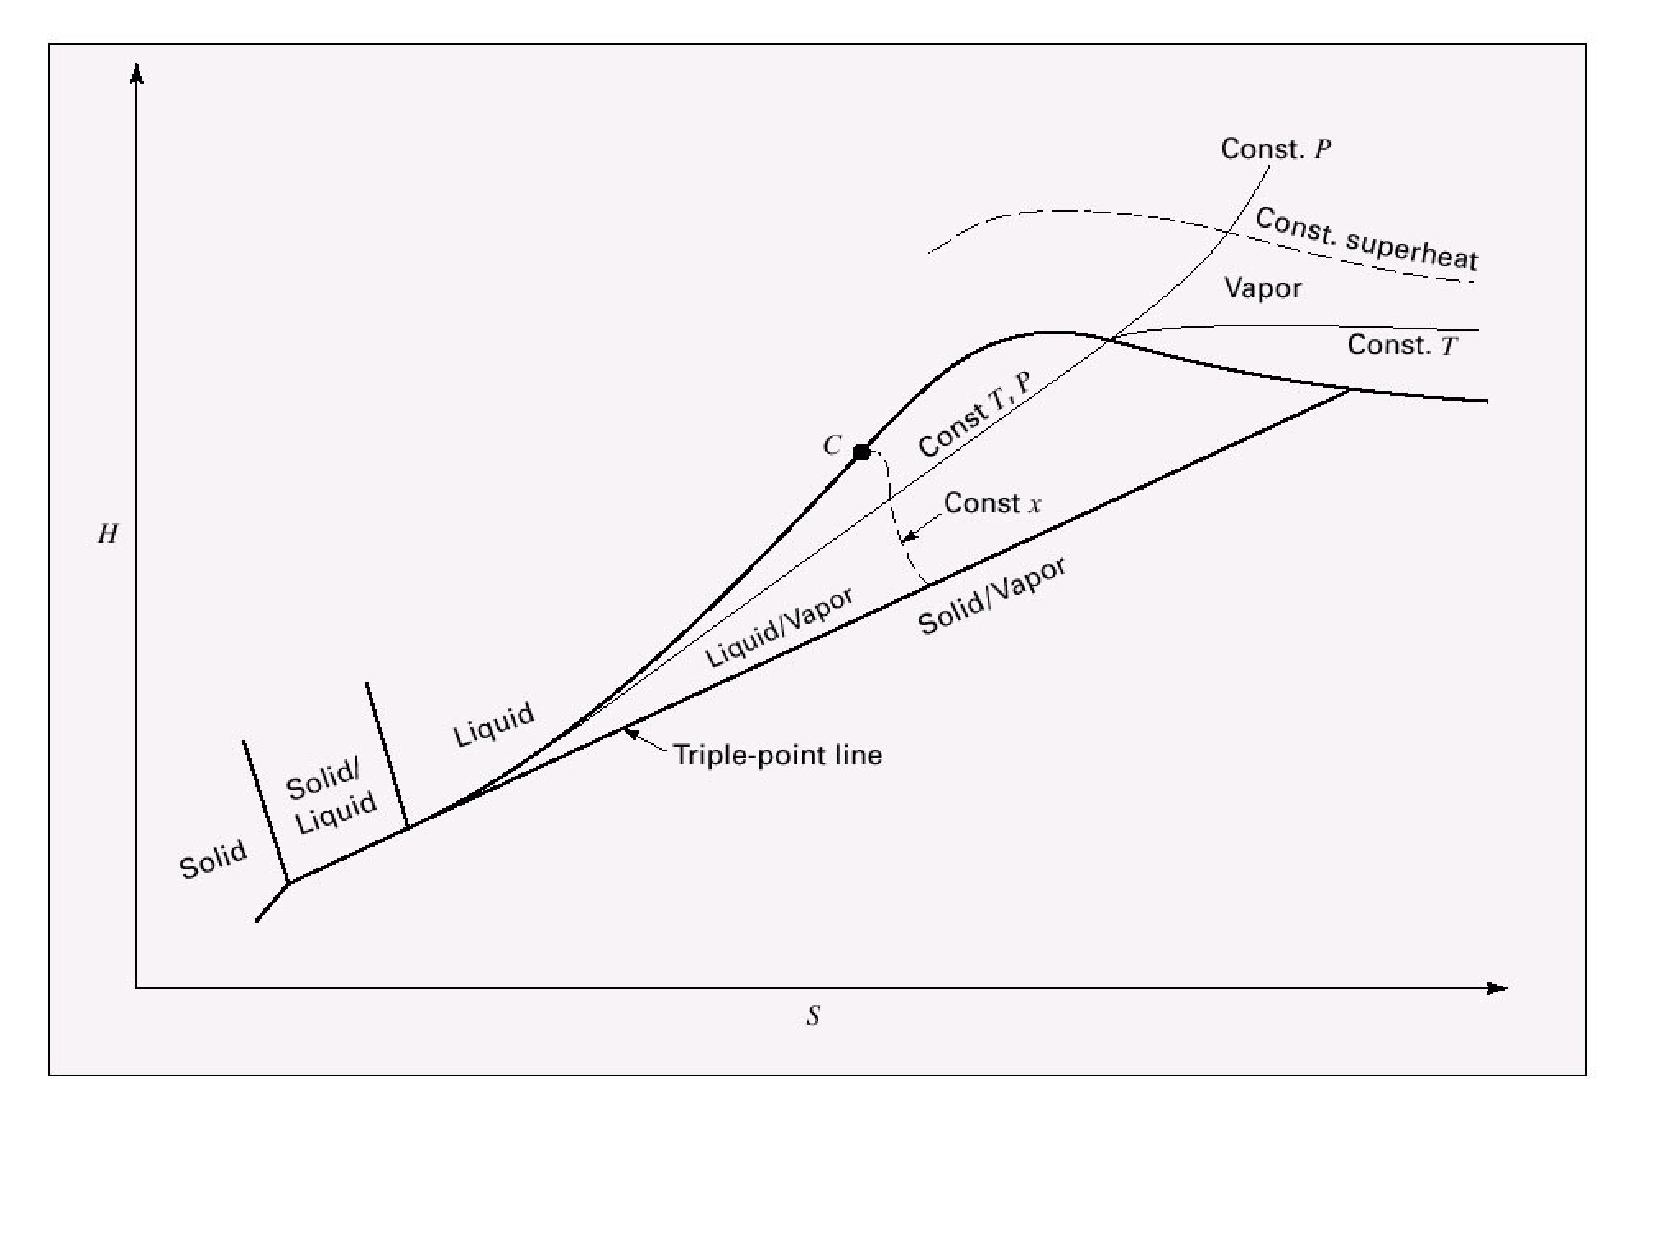
\includegraphics[width=1\columnwidth,clip]{./Pics/MoillerDiagram}
        \end{center}
      \end{figure}
\end{frame}
\normalsize


\section{Summary}

%%%
%%% Slide
%%%
%\scriptsize
\begin{frame}
 \frametitle{Summary}
   \begin{enumerate}[(i)]
     \item New thermodynamic potential properties: Gibbs and Helmholtz free energies;
     \item Introduction of Maxwell's relations and applications;
     \item Internal energy, enthalpy, entropy Gibbs and Helmholtz energies described as functions of pressure, volume and temperature (PVT);
     \item Introduction of residual properties and applications;
     \item Two-phase systems.
   \end{enumerate}
\end{frame}


\end{document}
 
